\NeedsTeXFormat{LaTeX2e}

\documentclass[a4paper,12pt]{pkg/monografia}
% \usepackage[pdfpagelabels]{hyperref}
\usepackage{amsmath,amsthm,amsfonts,amssymb}
\usepackage[mathcal]{eucal}
\usepackage{latexsym}
\usepackage[utf8]{inputenc}
% \usepackage[brazil]{babel}
%\usepackage{bm}
\usepackage[alf]{pkg/abntex2cite}
\usepackage{url}
\usepackage{enumitem}
\usepackage{graphicx}
\usepackage{placeins}
%\usepackage{epstopdf}
\usepackage{multirow}
%\usepackage{fancyhdr}
\usepackage[FIGTOPCAP]{subfigure}
\usepackage{textcase}
\usepackage{tabularx}
\usepackage[table,xcdraw]{xcolor}
% \usepackage{tlatex}
%\usepackage[portuguese,noend,ruled]{algorithm2e}
\usepackage{listings}
\usepackage[T1]{fontenc}
\usepackage{courier}
\usepackage[printonlyused]{acronym}
\usepackage{caption}
\usepackage{adjustbox}
\usepackage{floatrow}
\floatsetup[figure]{capposition=top}
\floatsetup[table]{capposition=top}
%\captionsetup{labelsep=endash}
%\usepackage{rotating}
%\usepackage{rotfloat}
%\usepackage{placeins}
% \usepackage{fontspec}B
% \setmonofont{Inconsolata}
%\captionsetup[listing]{position=top}
\usepackage{makecell}
\usepackage{listings}

%-----------------------------------------------------------
\begin{document}

%----------------- Título e Dados do Autor -----------------
\titulo{Tradução automática de especificação formal modelada em TLA+ para linguagem de programação}
\autor{Gabriela Moreira Mafra}
\nome{Gabriela Moreira}
\ultimonome{Mafra}

%---------- Informe o Curso e Grau -------------------------
\bacharelado \curso{Ciência da Computação} \mes{Março} \ano{2019}
\data{\today} % Data da aprovação
\cidade{Joinville}

%---------- Informações sobre a Instituição -----------------
\instituicao{Universidade do Estado de Santa Catarina}
\sigla{UDESC} \unidadeacademica{Centro de Ciências Tecnológicas}

%-- Nomes do Orientador, 1o. Examinador e 2o. Examinador ---
\orientador{Cristiano Damiani Vasconcellos}
\coorientador{Karina Girardi Rôggia}
\examinadorum{Adelaine Gelain}
\examinadordois{Paulo Torrens}
%\examinadortres{}

%-- Títulos do Orientador, 1o. Examinador e 2o. Examinador -
\ttorientador{Doutor}
\ttcoorientador{Doutora}
\ttexaminadorum{Mestre}
\ttexaminadordois{Mestre}
%\ttexaminadortres{}

%---------- Capa -------------------------------------------
\maketitle

%---------- Agradecimentos----------------------------------
%\agradecimento{Agradecimentos}
\section*{Agradecimentos}

Lorem ipsum dolor sit amet, consectetur adipisicing elit, sed do eiusmod tempor incididunt ut labore et dolore magna aliqua. Ut enim ad minim veniam, quis nostrud exercitation ullamco laboris nisi ut aliquip ex ea commodo consequat. Duis aute irure dolor in reprehenderit in voluptate velit esse cillum dolore eu fugiat nulla pariatur. Excepteur sint occaecat cupidatat non proident, sunt in culpa qui officia deserunt mollit anim id est laborum.

%\newpage

%---------- Epígrafe ---------------------------------------
%\begin{epigrafe}



%\end{epigrafe}

%---------- Resumo -----------------------------------------
\resumo{Resumo}
Lorem ipsum dolor sit amet, consectetur adipisicing elit, sed do eiusmod tempor incididunt ut labore et dolore magna aliqua. Ut enim ad minim veniam, quis nostrud exercitation ullamco laboris nisi ut aliquip ex ea commodo consequat. Duis aute irure dolor in reprehenderit in voluptate velit esse cillum dolore eu fugiat nulla pariatur. Excepteur sint occaecat cupidatat non proident, sunt in culpa qui officia deserunt mollit anim id est laborum.

\\
\noindent \textbf{Palavras-chaves:} Especificação de software, Lógica temporal, Geração de código, Métodos formais, Model checking

%---------- Abstract ---------------------------------------
\resumo{Abstract}
Specifying software provides safety guarantees for the system and
facilitates modifications and optimizations on the specified program, which is specially interesting for concurrent or distributed systems, where there are many behaviors to be considered. Specifications for this systems can be written in the specification language \TLAA, which is composed by definitions close to mathematics and tools that allow verification of temporal logic described properties. This work proposes an automatic translator of \TLA specifications to the funcional and concurrent programming language Elixir, allowing the execution of the specified system.

\\
\noindent \textbf{Keywords:} Software specification, Temporal Logic, Code Generation, Formal Methods, Model Checking

%-----------------------------------------------------------

% SUMÁRIO, LISTA DE FIGURAS E LISTA DE TABELAS
%---------- Sumário ----------------------------------------
\tableofcontents
\thispagestyle{empty}

%---------- Lista de figuras -------------------------------
\listoffigures
\thispagestyle{empty}

%---------- Lista de tabelas -------------------------------
\listoftables
\thispagestyle{empty}

%---------- Lista de Abreviaturas --------------------------
\listofabbreviations{Lista de Abreviaturas}
\begin{acronym}[]
	\acro{amqp}[AMQP]{{\it Advanced Message Queuing Protocol}}
	\acro{api}[API]{{\it Application Programming Interface}}
  \acro{aws}[AWS]{{\it Amazon Web Services}}
	\acro{cli}[CLI]{{\it Command Line Interface}}
	\acro{crud}[CRUD]{{\it Create Read Update Delete}}
	\acro{cpu}[CPU]{{\it Central Processing Unit}}
	\acro{cs}[C/S]{{Cliente/Servidor}}
	\acro{ddos}[DDoS]{{\it Distributed Denial of Service}}
	\acro{fps}[FPS]{{\it First-person shooter}}
	\acro{http}[HTTP]{{\it Hypertext Transfer Protocol}}
	\acro{iaas}[IaaS]{{\it Infrastructure as a Service}}
	\acro{ide}[IDE]{{\it Integrated Development Environment}}
	\acro{idl}[IDL]{{\it Interface Description Language}}
  \acro{ids}[IDS]{{\it Intrusion Detection System}}
	\acro{json}[JSON]{{\it JavaScript Object Notation}}
	\acro{jwt}[JWT]{{\it JSON Web Token}}
	\acro{kvm}[KVM]{{\it Kernel-based Virtual Machine}}
	\acro{lan}[LAN]{{\it Local Area Network}}
  \acro{ldap}[LDAP]{{\it Lightweight Directory Access Protocol}}
	\acro{mhz}[MHz]{{\it Mega-hertz}}
	\acro{mmo}[MMO]{{\it Massively Multiplayer Online}}
	\acro{mmofps}[MMOFPS]{{\it Massively Multiplayer Online First-Person Shooter}}
	\acro{mmorpg}[MMORPG]{{\it Massively Multiplayer Online Role-Playing Game}}
	\acro{moba}[MOBA]{{\it Multiplayer Online Battle Arena}}
	\acro{mvc}[MVC]{{\it Model-View-Controller}}
	\acro{nist}[NIST]{{\it National Institute of Standards and Technology}}
	\acro{npcs}[NPCs]{{\it Non-Playable Characters}}
	\acro{ntsc}[NTSC]{{\it National Television System Committee}}
	\acro{p2p}[P2P]{{\it Peer-to-Peer}}
	\acro{pvp}[PvP]{{\it Player vs Player}}
	\acro{pvnpc}[PvNPCs]{{\it Player vs \ac{npcs}}}
	\acro{paas}[PaaS]{{\it Platform as a Service}}
	\acro{pov}[POF]{{\it Point of View}}
	\acro{qos}[QoS]{{\it Quality of Service}}
	\acro{ram}[RAM]{{\it Random Access Memory}}
	\acro{rest}[REST]{{\it Representational State Transfer}}
	\acro{rpc}[RPC]{{\it Remote Procedure Call}}
	\acro{rpg}[RPG]{{\it Role-Playing Game}}
	\acro{rts}[RTS]{{\it Real-Time Strategy}}
	\acro{sdn}[SDN]{{\it Software Defined Network}}
	\acro{saas}[SaaS]{{\it Software as a Service}}
	\acro{snmp}[SNMP]{{\it Simple Network Management Protocol}}
	\acro{tcp}[TCP]{{\it Transmission Control Protocol}}
	\acro{tps}[TPS]{{\it Third-person Shooter}}
	\acro{tia}[TIA]{{\it Television Interface Adapter}}
	\acro{udp}[UDP]{{\it User Datagram Protocol}}
	\acro{vlan}[VLAN]{{\it Virtual Local Area Network}}
	\acro{vm}[VM]{{\it Virtual Machine}}
	\acro{vpn}[VPN]{{\it Virtual Private Network}}
	\acro{wan}[WAN]{{\it Wide Area Network}}
	\acro{ws}[WS]{{\it Web Services}}
	\acro{xdr}[XDR]{{\it External Data Representation}}
	\acro{xml}[XML]{{\it Extensible Markup Language}}



	\acrodefplural{vpn}[VPNs]{{\it Virtual Private Networks}}
	\acrodefplural{vlan}[VLANs]{{\it Virtual Local Area Networks}}
	\acrodefplural{vm}[VMs]{{\it Virtual Machines}}
\end{acronym}

% Defining: \acro{acronym}[short name]{full name}
% Usaging:
% \ac{acronym}     -- writes the full name followed by the acronym in brackets; later calls will write only the acronym
% \acf{acronym}     -- writes the full name followed by the acronym in brackets
% \acs{acronym}     -- writes the short name only
% \acl{acronym}     -- writes the full name only
% Use p at the end of previous commands for plural form (e.g., \acp for the plural form of \ac)
% \acresetall        -- reset usage of all acronyms (i.e., \ac will print full name again)
% \acused                -- mark the acronym as used

\thispagestyle{empty}

%---------- Início do Conteúdo -----------------------------
\pagestyle{ruledheader}

\chapter{Introdução}
\label{introducao}

Desde a década de 60, com os trabalhos de Floyd e Hoare, são feitos trabalhos com propostas para especificar software formalmente. Com especificações, o grau de confiança na correção do programa aumenta, e se torna possível provar formalmente algumas propriedades, com base na semântica da especificação.

Esses trabalhos, contudo, são direcionados a programas sequenciais. Especificar um software concorrente necessita uma modelagem diferente, e não era possível até os primeiros trabalhos de Leslie Lamport na década de 90.

Os métodos de especificação mais bem sucedidos são baseados em modelar transformações de estados com alguma lógica formal. Pensando em sistemas concorrentes, Lamport propõe uma lógica que estende os termos básicos da lógica temporal para permitir predicados sobre pares de estados, o que ele chama de ações. Essa abstração permite manipular ações e não o sistema temporal puro. Essa lógica é chamada de TLA - \textit{Temporal Logic of Actions}.

Sistemas concorrentes são aqueles onde mais de uma computação acontece no mesmo intervalo de tempo - concorrentemente - podendo ou não interagir entre si. Na lógica temporal, os passos executados por todas essas computações concorrentes são descritos como um comportamento, e definidos por uma sequência infinita de estados. Assim, uma fórmula da lógica pode ser verdadeira ou falsa para um comportamento, assim como pode ser válida ou não para todos os comportamentos possíveis.

Com essa abordagem, é possível verificar propriedades sobre um sistema especificado. Especificar um sistema significa definir todos os seus comportamentos possíveis. Tratando-se de um sistema concorrente, é esperado que existam muitos comportamentos, e listá-los exaustivamente seria uma tarefa extremamente passível de erro. Para viabilizar a definição dos comportamentos, é empregada uma modelagem semelhante a de uma máquina de estados, onde é definida a fórmula para o estado inicial e as fórmulas para as transições.

Baseando-se na lógica definida como TLA, Lamport propõe a linguagem de especificação formal \TLA (\textit{Temporal Logic of Actions}), com o objetivo de escrever provas formais para sistemas concorrentes da maneira mais simples possível~\cite{tlahistory}. Nessa linguagem, além dos operadores de TLA, são incluídos elementos da teoria de conjuntos e alguns açúcares sintáticos para fórmulas temporais como cláusulas \IF e \textsc{case}.

No viés de permitir verificações de propriedades, surge o \textit{model checker} TLC. Um \textit{model checker} busca todos os estados atingíveis de um modelo, de forma que todos os comportamentos possíveis são verificados. O TLC recebe uma especificação e uma configuração, e verifica se as fórmulas temporais dadas são válidas para a especificação. Se nenhuma fórmula temporal for dada, o TLC checará a presença de erros na semântica de \TLA e de situações de \textit{deadlock}. A checagem de \textit{deadlock} pode ser desativada, já que pode significar terminação em alguns sistemas.

Mais recentemente, outra ferramenta para verificar propriedades de uma especificação está em desenvolvimento : o sistema de provas TLAPS (\textit{TLA Proof System}) \cite{tlaps2010}. Esse sistema permite checar mecanicamente algumas provas, semelhantemente a Coq e Isabelle, mas ainda está incompleto.

A partir das definições de propriedades desejadas e da possibilidade de verificá-las, se torna possível alterar uma especificação no sentido de buscar por otimizações ou propostas diferentes para o sistema e, através das verificações, encontrar potenciais problemas como \textit{bugs} e inconsistências com as propriedades exigidas. Esses benefícios foram reportados pela \textit{Amazon Web Services} ~\cite{amazon}, que afirma ter usado TLA+ em 10 sistemas complexos e, para cada um deles, ter encontrado \textit{bugs} ou adquirido entendimento e confiança para implementar otimizações agressivas.

As especificações escritas, contudo, não possuem nenhum vínculo com a implementação se não pelo entendimento do programador que as escreveu. Outras linguagens de especificação formal com objetivos semelhantes ao TLA+, como Z, B-Method e ASM, fornecem formas de gerar código a partir do modelo. Contudo, até a data da escrita desse texto, não foram encontrados geradores de código a partir de modelos escritos em TLA+, impossibilitando a conversão das especificações em linguagens de programação com garantia de correspondência.

% Com o programa especificado, validado e traduzido para linguagem de programação, é possível aplicá-lo diretamente em casos reais com a garantia de correspondência e, portanto, das propriedades verificadas; ou então melhorar a implementação para uma versão mais otimizada, mas que parte da mesma base - nesse caso, a garantia é reduzida, já que as mudanças não estavam representadas no modelo original. Observações sobre os benefícios da geração de código a partir de modelos de especificação formal já foram verificadas em trabalhos como o estudo de caso em \cite{Leonard2008}.

\section{Objetivos}

Esse trabalho é feito com a intenção de elaborar um método de tradução, através do mapeamento de estruturas e construtores, de especificações formais descritas em TLA+ para código em linguagem de programação com possibilidade de ser executado e modificado; assim como implementar um tradutor que aplique esse método.

\subsection{Objetivos Específicos}
\begin{itemize}
  \item Encontrar mapeamentos entre as estruturas de especificação em TLA+ e estruturas de linguagens de programação
  \item Implementar um gerador de código Elixir, com capacidade de fazer \textit{parsing} de especificações em TLA+ e aplicar os mapeamentos necessários.
\end{itemize}

\chapter{\TLA}
\label{cap2}

\TLA é uma linguagem de especificação de software, criada por Leslie Lamport \cite{tlahistory} voltada à modelagem de sistemas concorrentes. Ela se propõe a oferecer uma maneira mais simples de escrever um algoritmo, ao utilizar um nível de abstração acima do que há ao escrever código em uma linguagem de programação. Assim, ao programar, não é necessário atentar-se a detalhes de implementação, permitindo o foco no comportamento do algoritmo - e não das suas dependências.

As especificações são descritas em fórmulas lógicas, com pequenas adaptações de sintaxe. Para facilitar a curva de aprendizado para engenheiros, foi criada a linguagem PlusCal \cite{pluscal}, com uma sintaxe semelhante a linguagens de programação imperativas, e que traduz seus programas para \TLA. A linguagem PlusCal não permite especificar sistemas tão complexos quanto os que podem ser escritos diretamente em \TLA, mas, devido à tradução para a linguagem original, aproveita completamente as capacidades dela de verificação de propriedades.

O método de especificação é baseado em máquinas de estados \cite{tlahistory} e, sendo assim, a descrição de um modelo é composta por uma condição inicial, que determina os possíveis estados inciais, e por uma relação de transições, que determina os possíveis estados que podem suceder cada estado em uma execução. Dessa forma, o conjunto de comportamentos especificado é composto por todos os comportamentos cujo estado inicial satisfaz a condição inicial e todas as transições fazem parte relação.

Lamport destaca \cite{hyperbook} que as especificações deveriam ser sobre modelos de uma abstração do sistema, e não algo retirado do próprio sistema. Semelhante à planta de um edifício, a especificação pode ser consultada para obter informações sobre o edifício (ou programa) de forma mais conveniente, além de ser capaz de facilitar uma série de verificações e perceber problemas enquanto a mudança ainda não é inviavelmente custosa.

Sendo assim, uma especificação em \TLA pode ser sobre comportamentos do ambiente no qual o programa funciona - como ao especificar um sistema e verificar possíveis comportamentos indesejáveis, entendendo aonde o programa deve atuar - des\-crevendo as operações existentes daquele sistema.

Não limitada a definição de um sistema, uma especificação pode incluir comportamentos do programa em si, compostas por operações existentes do sistema e novas operações definidas pelo programa. Em seu livro \cite{specifying-systems}, Lamport define um sistema de memória linear e, então, propõe uma implementação de um programa de escrita através de \textit{cache} que atua sobre um sistema de memória linear. Assim, ele verifica que a especificação da implementação dele satisfaz a especificação do sistema e prova a implementação. Nos exemplos deste capítulo, serão explicadas especificações de sistemas e de implementações.

\section{Lógica Temporal das Ações}

\TLA combina a Lógica Temporal das Ações, TLA (\textit{Temporal Logic of Actions}), proposta por Lamport em \cite{tlaformalization}, com teoria dos conjuntos - mais especificamente, a teoria de conjuntos de Zermelo-Fraenkel (ZFC), como detalhado em \cite{merzlogic}.

Lamport sumariza em \cite{proofsystem} o uso de TLA em \TLA. TLA é uma lógica temporal linear. Em \TLA, as variáveis rígidas do TLA são chamadas constantes, enquanto as flexíveis são chamadas variáveis. As constantes são declaradas com a palavra-chave \CONSTANTS e tem o mesmo valor para todos os estados de um comportamento - podendo diferir entre comportamentos. Já variáveis são declaradas com a palavra-chave \VARIABLES\ e podem ter valores diferentes em cada estado de um comportamento.

Os operadores são classificados em constantes e não constantes. Os constantes são aqueles que podem ser escritos em lógica clássica de primeira ordem. Os não constantes dependem de mais fatores, tal como o operador \textit{primed} ('), que depende do valor de uma variável em um estado diferente do atual. As definições em \TLA podem ser categorizadas em tipos de expressão. São denominadas fórmulas todas as expressões com valoração booleana.
\begin{itemize}
  \item \textbf{Expressões constantes} são expressões com apenas constantes declaradas e operadores constantes. Pela definição de operador constante, o valor de uma expressão constante depende apenas do valor das constantes contidas nela.
  \item \textbf{Expressões de estado} contém expressões constantes e variáveis declaradas. O valor de uma expressão de estado depende do estado, já que os valores das variáveis são definidos em um estado. Quando não são fórmulas, ou seja, sua valoração não é booleana, são chamadas também de funções de estado.
  \item \textbf{Expressões de ação} contém expressões de estado e operadores não constantes. O seu valor depende de um passo - um par de estados. Esse tipo de definição sobre ações dá o nome \textit{actions} a TLA, e pode ser chamado simplesmente de ação.
  \item \textbf{Expressões temporais} são permitidas apenas com valoração booleana em \TLA, sendo assim, chamadas sempre de fórmulas temporais. Elas contém expressões de ação os operadores $\square$ e $\Diamond$ da lógica temporal (definidos posteriormente neste capítulo). O valor de uma fórmula temporal depende de uma sequência de passos - um comportamento.
\end{itemize}

Com essa estrutura, define-se a sintaxe na Figura \ref{fig:sintaxe-tla}. A hierarquia permite que toda a complexidade das definições em uma especificação esteja nas fórmulas de ações. Os operadores temporais são usados somente no momento de verificar propriedades de segurança, vivacidade e razoabilidade (\textit{fairness}).

\begin{figure}[h]
  \centering
  \fbox{$\begin{array}{l} \begin{array}{lrll}
    \text{Constantes} & c & ~~~~
    \text{Variáveis} & v \\
    \text{Estados} & s, t & ~~~~
    \text{Funções de estado} & f, g \\
    \text{Conjuntos} & S \\
    \end{array} \\ \\
    \begin{array}{lrcl}
  \text{Ação} & \FANCYA & ::= & c \,\mid\, v \,\mid\, v' \,\mid\, \neg \FANCYA \,\mid\, \FANCYA \land \FANCYA \smallskip\\
  \text{Predicado} & P, Q & ::= & c \,\mid\, v \,\mid\, \neg P \,\mid\, P \land P \,\mid\, \ENABLED \FANCYA\smallskip\\
  \text{Fórmula Simples} & F & ::= & P \,\mid\, \square[\FANCYA]_f  \mid\, \square\langle\FANCYA\rangle_f \,\mid\,  \neg F \,\mid\,  F \land F  \,\mid\, \square F \smallskip\\
  \text{Fórmula Geral} & G & ::= & F \,\mid\, \EE x : G  \,\mid\, \neg G \,\mid\,  G \land G \mid\, G \implies G \smallskip\\
  \end{array} \end{array}$}
  \caption{Sintaxe da linguagem de TLA}
\label{fig:sintaxe-tla}
\end{figure}

Uma fórmula temporal em TLA é verdadeira ou falsa em um comportamento, que é definido por uma sequência infinita de estados. Uma fórmula é dita válida se e somente se ela é verdadeira para todos os comportamentos. Assim, a especificação de um sistema é dada por uma fórmula geral $G$ e representa um sistema cujo conjunto de comportamentos permitidos é igual ao conjunto de comportamentos que satisfazem $G$.

Implementação é representada através de implicação. Uma especificação dada pela fórmula $G_1$ implementa outra especificação dada por $G_0$ se e somente se qualquer sistema cujo conjunto de comportamentos satisfaz $G_1$ também satisfaz $G_0$, ou seja, a fórmula $G_0 \implies G_1$ é válida.

Em \cite{tlaformalization}, são definidas também notações auxiliares. A lista abaixo apresenta a definição e atribui um possível significado a possíveis operadores para fórmulas temporais:
\begin{itemize}
  \item $\square F$ ($F$ é sempre verdadeiro) para uma fórmula temporal $F$ é satisfeito por um comportamento se e somente se $F$ é verdadeiro para todos os sufixos (primeiro estado em um passo) do comportamento.

  \item $\Diamond F$ (Eventualmente F) é definido como $\neg \square \neg F$.

  \item $F \leadsto G$ (Em qualquer momento em que $F$ for verdadeiro, $G$ eventualmente será) é definido como $\square(F \implies \Diamond G)$

  \item $F \stackrel{+}\rightarrow G$ para fórmulas temporais $F$ e $G$ é verdadeiro para um comportamento se e somente se $G$ é verdadeiro, pelo menos, enquanto $F$ é.

  \item \EE $x : F$ para uma variável $x$ e uma fórmula temporal $F$ é satisfeito por comportamento se e somente se existem alguns valores a serem atribuídos a $x$ que produzem um comportamento que satisfaz $F$. Esse operador é uma especialização do quantificador existencial comum $\E$ porque ele asserte a existência de uma sequência infinita de valores para $x$, e não um único valor.

\end{itemize}

Para ações, são definidos ainda outros operadores:

\begin{itemize}
  \item $f'$ para uma função de estado $f$ é o valor de $f$ no final de um passo. Em outras palavras, para um passo composto pelo par de estados $s$ e $t$, $f'$ é o valor de $f$ para $t$. De forma semelhante, $P'$ para um predicado $P$ é o valor de $P$ para o estado final de um passo.

  \item A fórmula $\square [\FANCYA]_f$ para uma ação $\FANCYA$ e uma função de estado $f$ é satisfeita por um comportamento se e somente se cada passo do comportamento satisfaz \FANCYA ou mantém o valor de $f$ - ou seja, $\FANCYA \lor (f = f')$.

  \item A fórmula $\square \langle\FANCYA\rangle_f$ para uma ação $\FANCYA$ e uma função de estado $f$ é satisfeita por um comportamento se e somente se cada passo do comportamento satisfaz \FANCYA e altera o valor de $f$ - ou seja, $\FANCYA \land (f \neq f')$.

  \item \ENABLED \FANCYA (\FANCYA é ativável) para uma ação \FANCYA é um predicado cujo valor é verdadeiro para um estado $s$ se e somente se é possível fazer um passo \FANCYA partindo de $s$. Isto é, existe um estado $t$ tal que o passo formado pelo par $s$ e $t$ satisfaz \FANCYA.

  \item \UNCHANGED $f$ ($f$ não é modificado) para uma fórmula de estado $f$ em um passo (par de estados) é definido como $f' = f$  (o valor de $f$ no estado atual é igual ao valor de $f$ no próximo estado).

\end{itemize}

TLA conta com muitos operadores constantes, trazidos da matemática, da lógica, da teoria de conjuntos e de linguagens de programação. Abaixo, são apresentados os considerados menos triviais, sendo que a lista completa é definida em \cite{specifying-systems}.

\begin{itemize}

  \item \CHOOSE $x \in S : P$ (escolha algum $x$ pertencente ao conjunto $S$ que satisfaça $P$) para uma variável $x$ e um predicado $P$ resulta em algum valor de $x$ que satisfaz $P$ se \EE $x : P$ for verdadeiro. Sobre \CHOOSE, e possível afirmar que se \EE $x : P$ então $P(\CHOOSE x \in S : P)$ é verdadeiro, e que para todo predicado $Q$ tal que $Q \equiv P$, é verdade que $(\CHOOSE x \in S : P) = (\CHOOSE x \in S : Q)$.

  \item $f \EXCEPT ![v] = e$ para uma função $f$, um elemento de seu domínio $v$ e uma expressão $e$ resulta em uma cópia de $f$ exceto pelo valor $f[v]$ que é igual a $e$.

  \item $[h_1 \mapsto e_1, \dots, h_n \mapsto e_n]$ é uma estrutura do tipo registro (\textit{record}) onde $h_i$ são campos e $e_i$ são expressões constantes para os valores de $h_i$. O valor de um campo $h$ qualquer em um registro $r$ pode ser obtido por $r.h$, e o operador $r \EXCEPT !h = e$ funciona de forma semelhante ao definido no item anterior, retornando uma cópia de $r$ exceto pelo valor de $r.h$, que é $e$.

  % \item \ASSUME $c$ (assuma $c$) para uma fórmula constante $c$ define $c$ como verdadeiro. Esse operador não tem nenhum efeito nas definições de uma especificação, apenas pode facilitar a verificação de teoremas.
\end{itemize}

Finalmente, os operadores lógicos $\land$ e $\lor$ podem ser prefixados às expressões, sendo

\begin{center}
  $\begin{array}{lll}
\begin{array}{ll}
  \land\ e_1\\
  \vdots ~~~~ & \equiv ~~~~ e_1 \land \dots \land e_n\\
  \land\ e_n
\end{array} &
~~~~ e ~~~~ &
\begin{array}{ll}
  \lor\ e_1\\
  \vdots ~~~~ & \equiv ~~~~ e_1 \lor \dots \lor e_n\\
  \lor\ e_n
\end{array}
\end{array}$
\end{center}

\subsection{Passos balbuciantes}

Os passos balbuciantes (\textit{stuttering steps}) são parte importante das especificações em TLA. Eles permitem que o estado - formado pelos valores das variáveis da especificação - se mantenha igual durante um passo.

Supondo que as variáveis da especificação estejam declaradas como
\[vars = \langle var_1, var_2, \dots, var_n\rangle\]

Então é possível usar o operador $\square [\FANCYA]_f$ definido, com $f = vars$, no seguinte teorema sobre uma especificação $Spec$

\[\THEOREM Spec \implies \square [\FANCYA]_{vars}\]

o que, se verificado, garante que cada passo de um comportamento satisfeito por $Spec$ satisfaz a ação \FANCYA ou é um passo balbuciante e mantém os valores das variáveis em $vars$. Isso é importante porque possibilita que nem todos os passos do sistema sejam especificados - seria muito complexo definir tudo o que pode ocorrer durante sua execução. Assim, definem-se apenas os passos relevantes para o sistema, e todos os outros passos - aqueles que não alteram as variáveis definidas - são permitidos. Um comportamento que passa a ter infinitos passos balbuciantes pode significar uma execução do sistema que finalizou. Com a definição de passos balbuciantes, é possível definir as propriedades apresentadas na Seção \ref{propriedades}.

\section{Propriedades}
\label{propriedades}

Sobre uma especificação definida, \TLA permite a verificação de algumas propriedades de segurança e vivacidade. Essas propriedades são descritas em forma de teoremas na especificação apenas com o intuito de documentar sua verificação, porém devem ser inseridas manualmente no modelo TLC para serem, de fato, checadas.

Propriedades são fórmulas temporais sobre ações definidas na especificação. Uma propriedade é satisfeita se a fórmula temporal que a define é válida.

\subsection{Propriedades de Segurança}

Propriedades de segurança define o que o sistema pode fazer. Quando uma propriedade de segurança é violada, ela é violada em um instante específico de um comportamento. Esse tipo de propriedade é definido em \TLA como uma invariante.

Uma invariante é um predicado $P$ que é verdadeiro em todos os passos de todos os comportamentos permitidos por uma especificação $Spec$, e pode ser verificada com a prova do teorema

\[\THEOREM Spec \implies \square P\]

\subsection{Propriedades de Vivacidade}

Propriedades de vivacidade definem o que o sistema deve fazer. Quando uma propriedade de vivacidade é violada, ela é violada em um comportamento. Em \cite{specifying-systems}, é apresentada uma especificação para um relógio. O ponteiro de um relógio deve, eventualmente, mexer. Esse é um tipo de propriedade que pode ser descrita com uma propriedade de vivacidade, tal qual a razoabilidade fraca (\textit{weak fairness}).

A razoabilidade fraca para uma fórmula de estado $f$ e uma ação \FANCYA é escrita como $WF_f (\FANCYA)$. Ela é satisfeita por um comportamento se e somente se \FANCYA $\land\ (f' \neq f)$ é infinitamente não ativável (\textsc{enabled}) ou infinitos passos \FANCYA $\land\ (f' \neq f)$ ocorrem. Sendo assim, essa propriedade garante que \FANCYA não possa permanecer continuamente ativável para sempre sem que um passo \FANCYA ocorra. Essa condição pode ser escrita de forma equivalente como

\[\square (\ENABLED \FANCYA \implies \Diamond\langle\FANCYA\rangle_f)\]

A conjunção com $(f' \neq f)$, expressada com a notação $\langle\FANCYA\rangle_f$, se deve ao fato de não ser desejável exigir que passos balbuciantes eventualmente ocorram. \FANCYA $\land\ (f' \neq f)$ pode ser lido como "todos os passos não balbuciantes que satisfazem \FANCYA".

A razoabilidade fraca recebe a denominação "fraca" porque exige que uma ação permaneça continuamente ativável para garantir a ocorrência de um passo satisfazendo-a. Se um comportamento repetidamente tornar a ação ativável e em seguida não ativável, a razoabilidade fraca não garante nada sobre a ocorrência da ação neste comportamento. Para tal, é necessário garantir a propriedade de razoabilidade forte (\textit{strong fairness}).

A razoabilidade forte para uma fórmula de estado $f$ e uma ação \FANCYA é escrita como $SF_f (\FANCYA)$ . Ela é satisfeita por um comportamento se e somente se \FANCYA $\land (f' \neq f)$ ocorre finitas vezes ou infinitos passos \FANCYA $\land (f' \neq f)$ ocorrem. Essa propriedade garante que \FANCYA não possa ser repetidamente ativável para sempre sem que um passo \FANCYA ocorra.Uma forma equivalente de representar essa condição é

\[\square \Diamond \ENABLED \FANCYA \implies \square \Diamond\langle\FANCYA\rangle_f\]

que pode ser lida como "se sempre \FANCYA for eventualmente ativável, então sempre um passo $\langle\FANCYA\rangle_f$ deve eventualmente ocorrer".

\section{Exemplo 1 - Jarros de Água}
\label{exemplo1}

Para exemplificar uma especificação de um sistema, é possível definir um problema combinatório simples como o dos jarros de água. Nesse problema, são fornecidos dois jarros inicialmente vazios, um com capacidade de 3 litros e outro com capacidade de 5 litros, assim como uma fonte inesgotável de água. Sendo assim, é possível despejar a água dos jarros no chão, transferir a água de um jarro ao outro ou encher um jarro com a fonte de água.

O objetivo do problema é ter exatamente 4 litros de água em um dos jarros. Isso é, dada uma máquina de estados, é necessário encontrar uma sequência de transições que leva a algum estado onde o jarro maior tem exatamente 4 litros de água. No entanto, para esse exemplo, deseja-se apenas especificar os comportamentos do sistema em si, e não de um possível programa que buscaria atingir esse objetivo. Uma possível especificação em \TLA para esse sistema se encontra na Figura \ref{fig:ex1tla}.

\begin{figure}
  \centering
  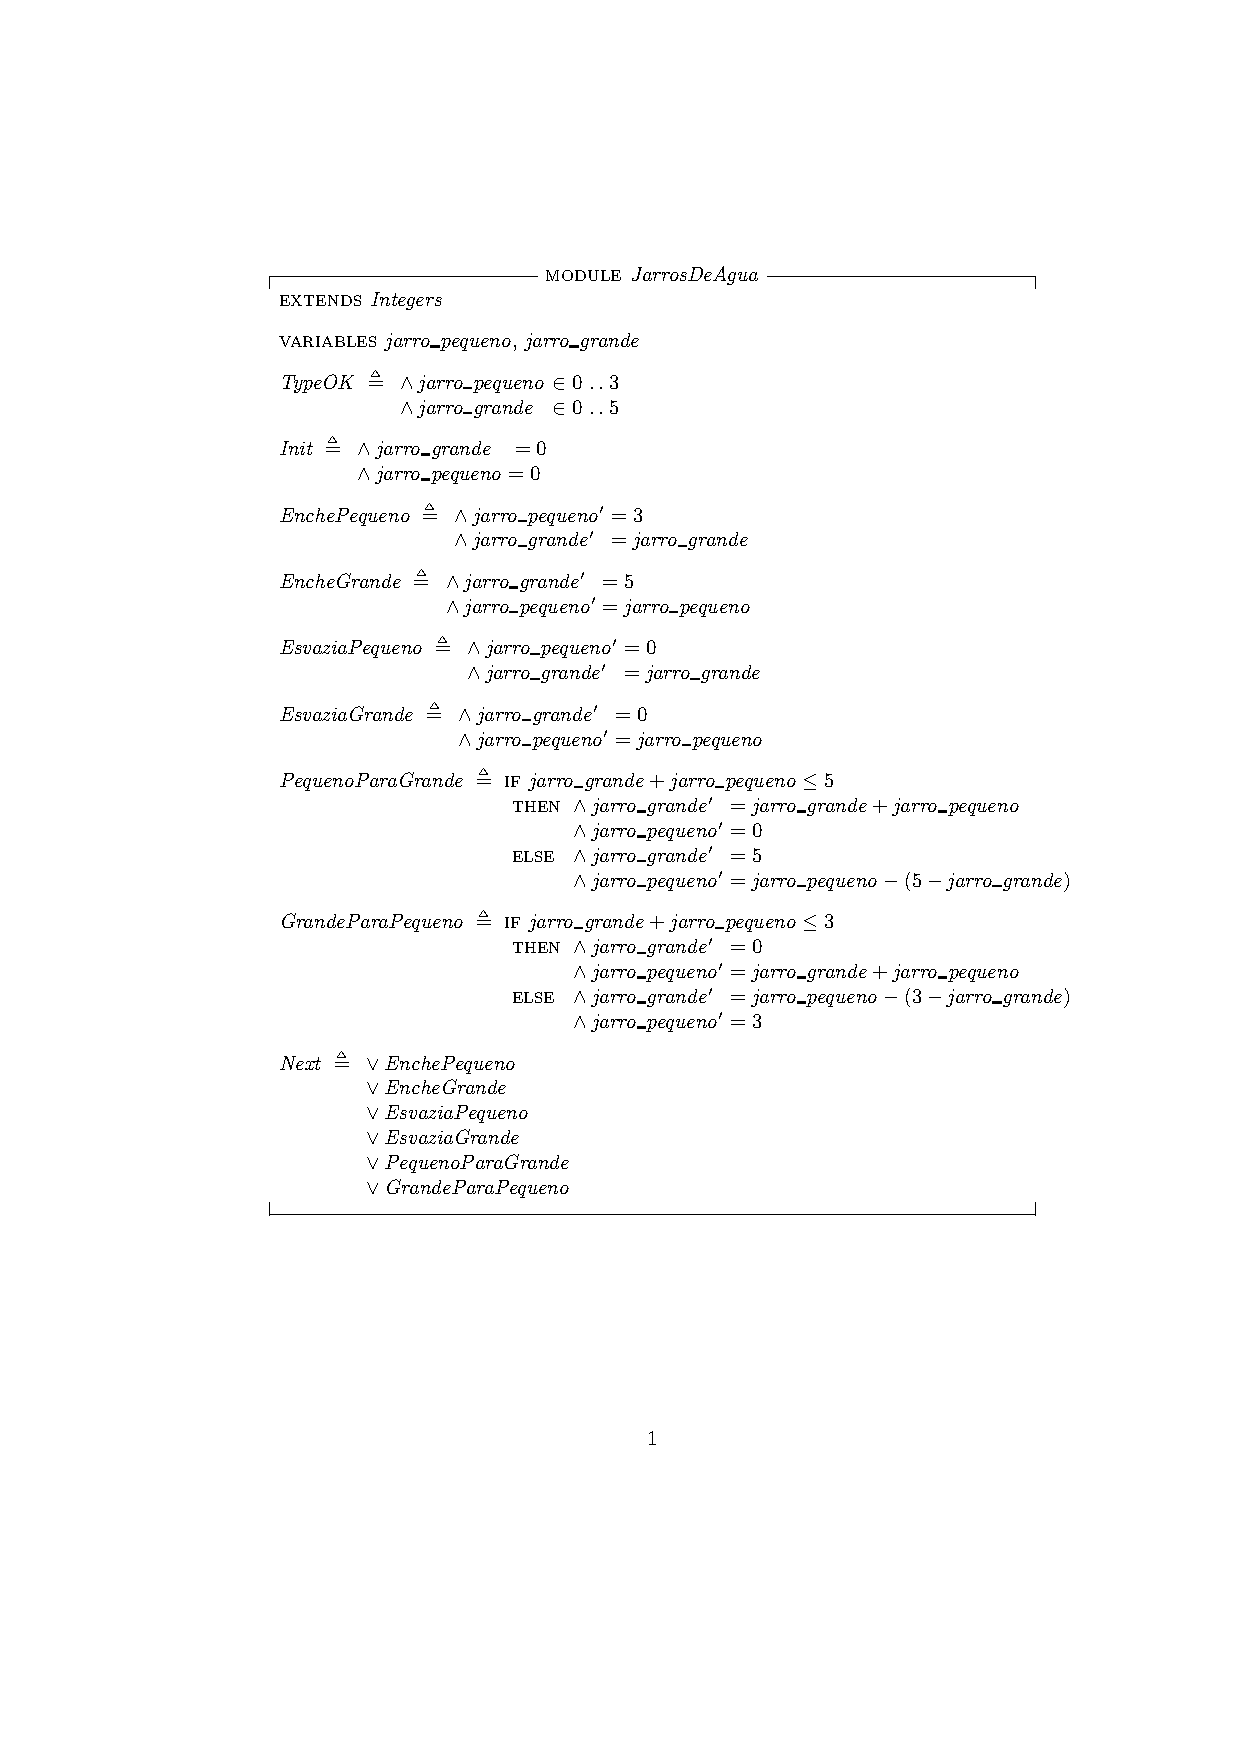
\includegraphics[width=\textwidth]{JarrosDeAgua.png}
  \caption{Especificação do problema dos Jarros de Água}
  \label{fig:ex1tla}
\end{figure}

Entendendo essa especificação no modelo de máquina de estado, é possível observar que as variáveis (\VARIABLES) são um conjunto de valores que variam nos estados, de forma que o conjunto com todas as combinações dos valores possíveis para cada uma das variáveis forma o conjunto de estados da máquina. Um estado desse sistema seria $jarro\_pequeno = 0, jarro\_grande = 1$. Na definição $Init$, é especificada uma fórmula que determina estados iniciais válidos - o que, nesse caso, é apenas o estado onde todas as variáveis do sistema tem valor 0.

As seis definições seguintes representam as transições através de ações. Em cada uma delas, as variáveis com o símbolo de linha representam os valores no estado seguinte, e sempre precisam ser definidas. Na transição $EnchePequeno$, o valor de $jarro\_grande$ se mantém o mesmo entre os estados atual e seguinte, mas é necessário explicitar isso com $jarro\_grande' = jarro\_grande$. Essa necessidade vem da aproximação da sintaxe de \TLA com a matemática, onde não existe efeito colateral e, portanto, o valor da variável $jarro\_grande$ não propaga de um estado para outro.

É possível, sintaticamente, utilizar a informação das variáveis do estado atual para definir o estado seguinte - não é necessário definir exaustivamente transições para todas as combinações de variáveis. Dessa forma, as ações definidas representam transições para vários estados do sistema. Cada transição da especificação do problema dos jarros pode ser aplicada nos em qualquer um dos estados, isto é: $(jarro\_pequeno = 0,\ jarro\_grande = 0), (jarro\_pequeno = 0,\ jarro\_grande = 1), \dots$.

No sentido de aproveitar informações do estado atual, é possível utilizar condicionais, como nas ações $PequenoParaGrande$ e $GrandeParaPequeno$. Com isso, é fácil definir transições diferentes para conjuntos de estados com propriedades diferentes. Na definição de $PequenoParaGrande$, os estados que atualmente possuem 5 litros ou menos de água nos jarros em total recebem uma transição para um estado onde o jarro pequeno está vazio. Já os estados que possuem mais de 5 litros de água recebem uma transição para um estado onde o jarro grande está cheio.

Ao fim dessa especificação, em $Next$, é definida a \textit{next state function} (função de próximo estado), na qual são declaradas as fórmulas transicionais do sistema, incluindo qualquer composição dessas fórmulas que possa levar um estado a outro. No caso do problema dos jarros, apenas é definido que qualquer transição pode ser utilizada para obter um novo estado.

As definições $Init$ e $Next$ são buscadas pelo \textit{model checker} TLC na construção da máquina de estados. É possível renomear essas definições, mas é preciso informar ao TLC os novos nomes para o estado inicial e a \textit{next state function}. A especificação - chamada $Spec$ - é descrita a partir dessas definições com a seguinte fórmula temporal:

\[Spec \defeq Init \land \square [Next]_{vars}\]

Onde $vars$ é uma tupla contendo todas as variáveis declaradas. Com essa especificação, o sistema está definido. As operações permitidas e as variáveis relevantes foram descritas e, a partir do estado inicial, cada passo do sistema pode ser executado a partir de uma das seis diferentes ações ou de passos balbuciantes sobre $vars$. Essas informações são suficientes para o TLC fazer verificações sobre o sistema, é apenas necessário definir tais verificações.

A definição $TypeOK$ na especificação apresentada pode ser utilizada para verificar os tipos desse sistema. Ela define que a variável $jarro\_pequeno$ é sempre um inteiro entre 0 e 3, e a variável $jarro\_grande$ é sempre um inteiro entre 0 e 5. Ou seja, $TypeOK$ será verdadeiro se e somente se os valores das variáveis estiverem de acordo com essas restrições. Isso não é uma verificação em si, e sim uma definição. Para que essa definição seja verificada em todos os estados alcançáveis pelo sistema, é necessário adicioná-la como uma invariante do modelo. Como uma invariante, o valor dela não deve ser modificado em nenhum estado da execução. Já que o estado inicial definido em $Init$ faz $TypeOK$ verdadeiro, ao colocar essa invariante, todos os estados devem fazer $TypeOK$ verdadeiro, ou o TLC retornará um erro. $TypeOk$ pode ser definido como uma invariante através do teorema:

\[\THEOREM Spec \implies \square (TypeOK)\]

Outra propriedade interessante de ser verificada para esse problema antes da implementação de um programa para resolvê-lo é a possibilidade de resolução, isto é, se é possível alcançar um estado onde onde o jarro maior contém 4 litros de água. Para isso, define-se uma invariante para o predicado $jarro\_grande\ \backslash= 4$, que não será satisfeita. Como esse predicado é verdadeiro para o estado inicial, o fato de ele não ser satisfeito significa que, em algum momento da execução, o predicado foi falso, ou seja, $jarro\_grande = 4$. Adicionando essa invariante, um possível teorema seria:

\[\THEOREM Spec \implies \square (TypeOK \land jarro\_grande\ \backslash= 4)\]

O TLC, ao encontrar uma execução que insatisfaz a invariante, traz a sequência de transições que levam ao estado onde o predicado é falso, o que, no caso do simples problema dos jarros, é a solução buscada.

Esse exemplo é apresentado com o intuito de demonstrar a estrutura da especificação de um sistema e o funcionamento das invariantes. A seguir, é proposto um exemplo com a especificação de um sistema real que pode ser implementado por especificações de programas para verificar que as propriedades definidas são mantidas. % e de um protocolo implementado sobre ele.

\section{Exemplo 2 - Transações em Bancos de Dados}
\label{exemplo2}

Já tratando de um contexto de um problema real de sistemas concorrentes, define-se uma especificação para o problema da consistência das transações em bancos de dados. Esse é um problema clássico onde, dado um conjunto de gerenciadores de recursos fazendo operações sobre um mesmo banco, um gerenciador só pode cometer (fazer a ação \textit{commit}) se todos os outros gerenciadores estiverem preparados para cometer, e se algum gerenciador quiser abortar, então todos devem abortar. Ou seja, em nenhum momento pode haver um gerenciador abortado e outro cometido.

\subsection{O sistema}

Na Figura \ref{fig:ex2tla}, encontra-se uma especificação para um sistema de transações consistente. Ela não apresenta uma proposta de solução para o problema, e sim traz uma descrição formal do que significa ser consistente quando se trata de transações. Uma especificação de uma solução para o problema deve implementar essa especificação.

\begin{figure}[h]
  \centering
  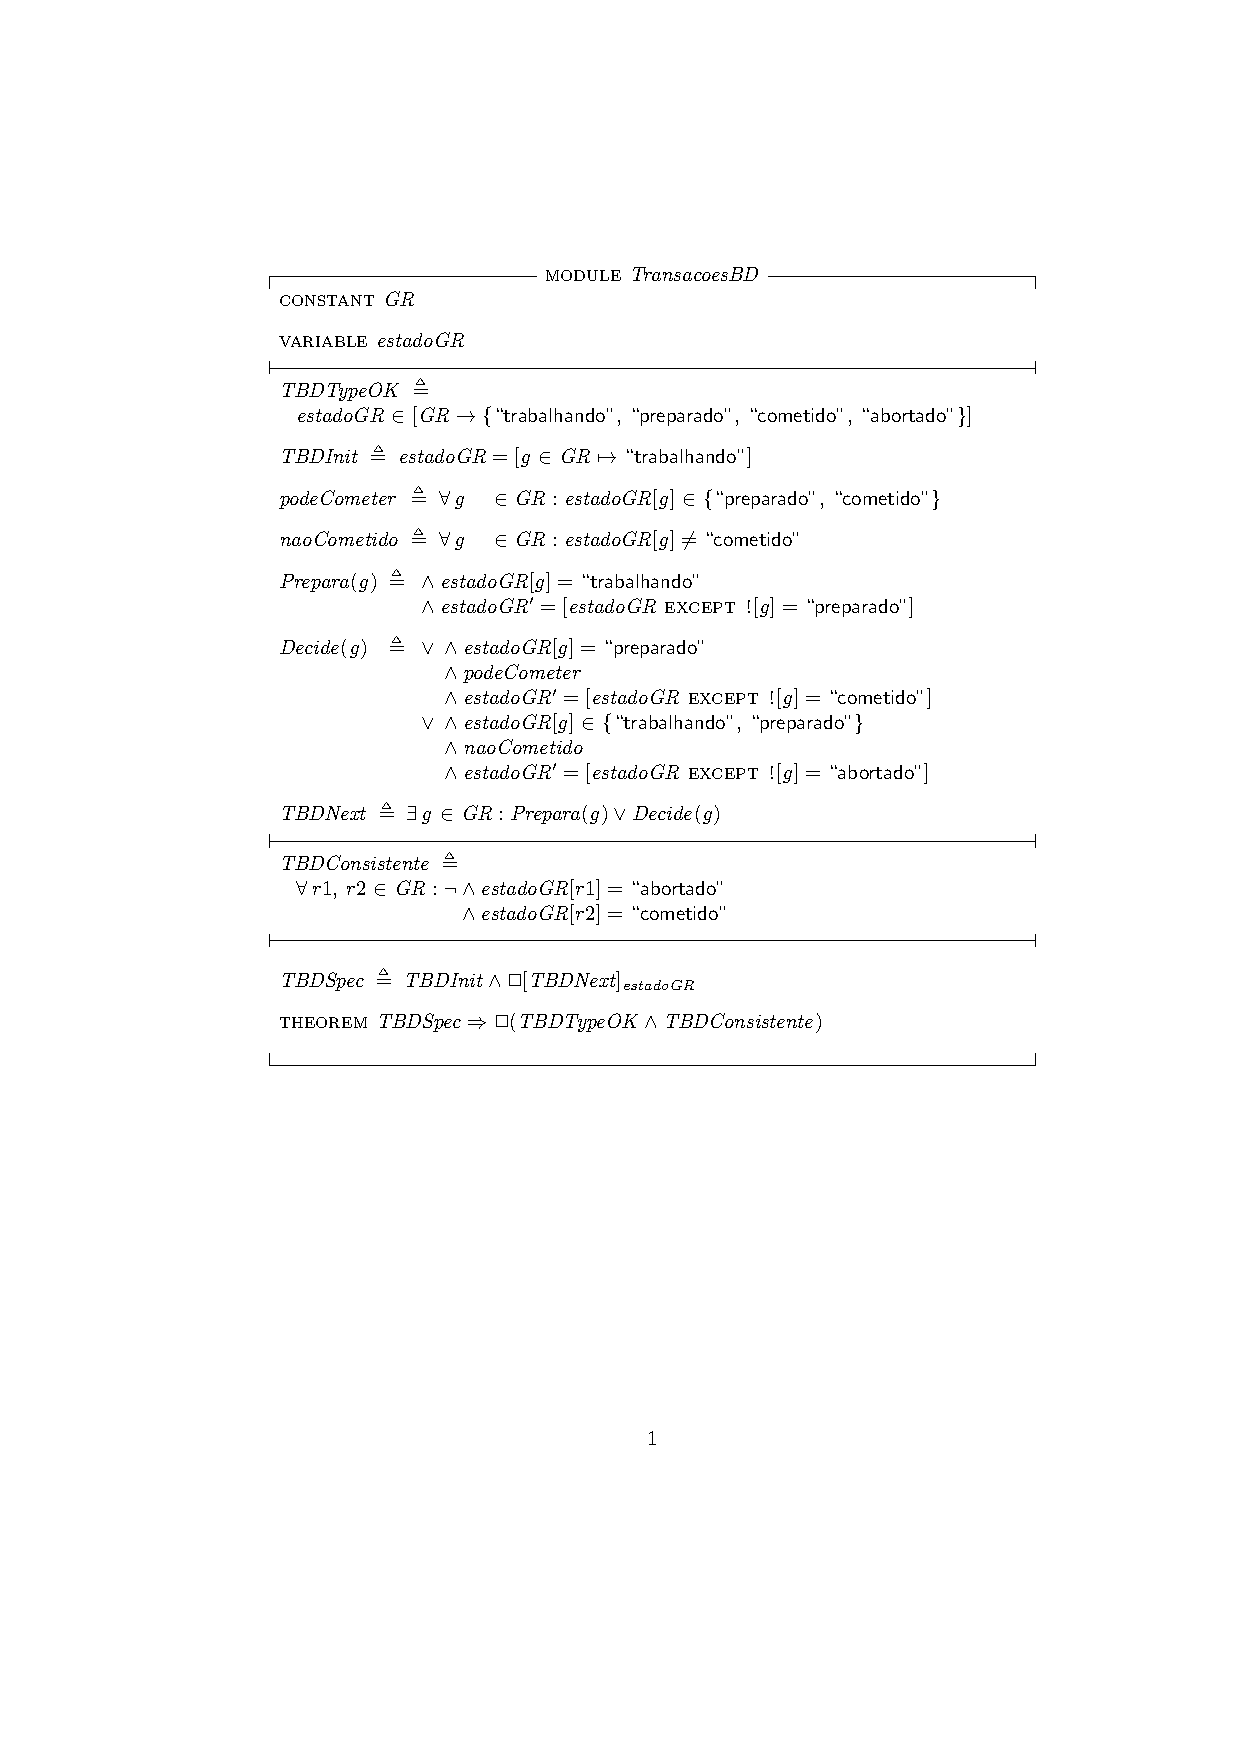
\includegraphics[width=\textwidth]{TransacoesBD.png}
  \caption{Especificação de um sistema de transações em bancos de dados}
\label{fig:ex2tla}
\end{figure}

Um gerenciador de recursos pode estar em quatro estados diferentes, como definido em $TBDTypeOK$. Do estado \trabalhando, ele pode ir para o estado \preparado, no sentido de que ele está pronto para cometer; ou então abortar, indo para o estado \abortado. Se todos os gerenciadores estão no estado \preparado, então qualquer um deles pode cometer, indo para o estado \cometido; ou então abortar, indo para o estado \abortado. Contudo, se exite algum gerenciador no estado \cometido, então nenhum outro gerenciador pode abortar.

A possibilidade de um gerenciador $g$ ir do estado \trabalhando\ ao \preparado\ é representada pela ação $Prepara(g)$ onde, se o estado de $g$ é \trabalhando, então o valor da variável $estadoGR$ no novo estado é igual ao seu valor no estado atual, exceto pelo valor de $estadoGR[g]$, que passa a ser \preparado.

A decisão de um gerenciador de abortar ou cometer é representada pela ação $Decide(g)$. Nessa definição, as fórmulas $podeCometer$ e $naoCometido$ são definidas separadamente para minimizar a complexidade cognitiva da especificação - definí-las dentro de $Decide(g)$ seria semanticamente equivalente. $podeCometer$ verifica se todos os estados estão preparados ou cometidos, ou seja, qualquer um pode cometer. Se $podeCometer$ for verdadeiro, e $g$ ainda não cometeu, então $g$ comete - o estado dos gerenciadores passa a ser uma cópia do estado atual exceto por $estadoGR[g]$, que é \cometido. Outra decisão possível, separada da primeira por um operador de disjunção, é a de abortar. Para isso, verifica-se, com a fórmula $naoCometido$, se não há nenhum gerenciador cometido. Se $naoCometido$ for verdadeira, e $g$ ainda não tiver abortado, então o novo estado dos gerenciadores passa a ter $g$ como \abortado.

Com essas fórmulas, é possível definir a \textit{next state function} $TBDNext$, onde um passo do sistema é dado por um gerenciador de recursos no conjunto $GR$ que faz uma ação de preparar ou decidir. A fórmula temporal $TBDSpec$ consiste a especificação do sistema de transações bancárias e tem um formato semelhante à fórmula $Spec$ do exemplo anterior, na Seção \ref{exemplo1}.

Para verificar que o sistema especificado por $TBDSpec$ está de acordo com a restrição do problema - em nenhum momento pode haver um gerenciador abortado e outro cometido - define-se $TBDConsistente$ onde, para cada possível par de gerenciadores de recursos, não é o caso de o primeiro estar abortado e o segundo, cometido. Essa fórmula é uma afirmação sobre um valor da variável $estadoGR$, porém precisa ser verdadeira para todos os valores dessa variável em qualquer comportamento que satisfaça $TBDSpec$. Para isso, ela é definida como uma invariante através do teorema

\[\THEOREM TBDSpec \implies \square(TBDTypeOK \land TBDConsistente)\]

que permite verificar que, se um comportamento satisfaz $TBDSpec$ - isto é, seu estado inicial satisfaz $TBDInit$ e seus passos satisfazem $TBDNext$ - então as fórmulas de estado $TBDTypeOK$ e $TBDConsistente$ são verdadeiras para todas as estados - todos os valores atribuídos para as variáveis - neste comportamento. Sendo satisfeito esse teorema, $TBDTypeOK$ e $TBDConsistente$ são ambos invariantes da especificação.

% \subsection{A implementação}

\chapter{O gerador de código}
\label{cap3}

Dada uma especificação na linguagem \TLA, contendo elementos da lógica TLA e da teoria de conjuntos, além de elementos sintáticos próprios, deseja-se obter uma definição equivalente em linguagem de programação. Equivalência para esse propósito é definida pela igualdade do conjunto de comportamentos permitidos. Isto é, todo comportamento especificado deve ser permitido na execução do código, e todo comportamento permitido pela execução do código deve ter sido especificado.

\section{Elixir}

Para esse propósito, a linguagem de programação escolhida para o código traduzido foi Elixir. As motivações são expostas abaixo por ordem de relevância na decisão:
\begin{enumerate}
  \item A concorrência é facilitada por ter seu código traduzido para \textit{bytecode} da máquina virtual do Erlang (BEAM). Suporte a concorrência é de extrema importância, já que \TLA foi criado para facilitar a especificação de sistemas concorrentes. É necessário que o código gerado seja capaz de refletir o sistema também nesse quesito.

  \item Uma linguagem funcional tende a se aproximar mais de definições matemáticas do que linguagens de outros paradigmas. Uma vez que a estrutura de \TLA foi construída principalmente no âmbito da matemática, a complexidade das traduções tende a ser menor para uma linguagem funcional.

  \item O alto nível de abstração da sintaxe de Elixir, que se inspira em Ruby e sua busca por código facilmente entendível, faz com o programador que trabalhar com o código gerado possa entendê-lo de forma mais simples e rápida do que seria com uma linguagem de baixo nível. Com isso, otimizações podem ser feitas com mais segurança, e a manutenabilidade do código é favorecida.

  \item A transparência de plataforma provida pela máquina virtual BEAM maximiza o número de ambientes aonde o código pode ser executado. Não seria de muito uso gerar um código para um ambiente específico, e uma máquina virtual permite que o código gerado seja \textit{Cross Plataform}.

  \item O seu código é aberto sobre a licença Apache 2.0, permitindo que o funcionamento de suas estruturas possa ser verificado a qualquer momento. Não seria possível garantir nenhuma correspondência do código gerado com a especificação se não fosse conhecida a execução gerada pelos operadores usados no código.

\end{enumerate}

Essa escolha vem de encontro com a finalidade de proporcionar um código modificável, de forma que o programador seja capaz de entender a correspondência entre as duas partes e minimizando a diferença do nível de abstração no qual ele está programando.

\section{A tradução}

A geração de código para uma especificação se dá pela tradução das estruturas de \TLA para Elixir. Esta tradução será feita de forma automática por uma ferramenta escrita em Haskell, implementada durante o corrente trabalho. A ferramenta será responsável pelo \textit{parsing} do aquivo da especificação, no formato \texttt{.tla}, para estruturas internas e, então, transformação dessas estruturas internas em código Elixir.

A escolha da linguagem Haskell para implementação do gerador de código é motivada pela possibilidade da definição de tipos algébricos generalizados, que facilitam na representação das estruturas, e na tipagem forte, que ajuda a garantir consistência das relações entre estruturas definidas durante o processo, minimizando a possibilidade de erros no desenvolvimento. Haskell também conta com a biblioteca de \textit{parsing} Parsec, que abstrai a complexidade de analisar sintaticamente um arquivo.

O escopo da tradução se limita à especificação definida, sendo suficiente para gerar código executável para o sistema definido. Traduzir teoremas e suposições não é necessário, uma vez que essas estruturas servem para fazer verificações sobre a especificação e não são necessárias para seu funcionamento. Ao código gerado não é atribuída a responsabilidade de refazer verificações, e sim de manter as propriedades já verificadas.

\subsection{Mapeamentos}

A tradução funciona como um grande mapeamento do conjunto de todas as especificações para um conjunto de programas em Elixir. Para viabilizar esse mapeamento, são definidos sub-mapeamentos que traduzem frações de uma especificação. Encontrar sub-mapeamentos suficientes para atender todo o domínio de especificações é suficiente para definir o processo de tradução.

Os primeiros mapeamentos definidos envolvem fórmulas transicionais e variáveis. Para cada fórmula transicional da especificação, é definida uma função, declarada com a sintaxe \texttt{def nome(parametros) do ... end}, que recebe as variáveis como parâmetro. O conjunto de variáveis do sistema é representado em uma Hash - estrutura de dados chave-valor de Elixir, equivalente a um dicionário - representada no padrão \texttt{variaveis = \%\{ variavel1: valor1, variavel2: valor2 \}} e podendo ser acessada com \texttt{variaveis[:variavel1]} para obter o valor.

Cada função mapeada de uma fórmula transicional recebe uma hash representando o estado atual e retorna outra hash representando o novo estado. O retorno, em Elixir, não exige uma palavra chave - a função retorna aquilo que a última linha retornou, sendo, para as funções geradas, a hash resultante da chamada do seu construtor.

A Figura \ref{fig:esvaziapequeno-elixir} contém a função mapeada da fórmula $EsvaziaPequeno$ definida na Figura \ref{fig:ex1tla}.

\begin{figure}[h]
  \centering
  $\progfig{
  ~~def esvazia\_pequeno(variaveis) do\\
  ~~~~\%\{\\
  ~~~~~~pequeno: 0,\\
  ~~~~~~grande: variaveis[:grande]\\
  ~~~~\}\\
  ~~end
  }$
  \caption{Fórmula transicional $EsvaziaPequeno$ como uma função em Elixir}
\label{fig:esvaziapequeno-elixir}
\end{figure}

Alguns operadores de \TLA permitem mapeamentos ainda mais diretos, como \IF e \CASE, devido a sua inspiração em linguagens de programação. A Figura \ref{fig:pequenoparagrande-elixir} traz a função correspondente à fórmula $PequenoParaGrande$ definida na Figura \ref{fig:ex1tla}. A sintaxe para operadores \IF em Elixir é na forma \texttt{if condição do ... else ... end}.

\begin{figure}[h]
  \centering
  $\progfig{
  ~~def pequeno\_para\_grande(variaveis) do\\
  ~~if variaveis[:grande] + variaveis[:pequeno] <= 5 do\\
  ~~~~~~\%\{\\
  ~~~~~~~~pequeno: 0,\\
  ~~~~~~~~grande: variaveis[:grande] + variaveis[:pequeno]\\
  ~~~~~~\}\\
  ~~~~else\\
  ~~~~~~\%\{\\
  ~~~~~~~~pequeno: variaveis[:pequeno] - (5 - variaveis[:grande]),\\
  ~~~~~~~~grande: 5\\
  ~~~~~~\}\\
  ~~~~end\\
  ~~end
  }$
  \caption{Fórmula transicional $PequenoParaGrande$ como uma função em Elixir}
\label{fig:pequenoparagrande-elixir}
\end{figure}

Com o conjunto inicial de mapeamentos apresentado, é possível definir todas as fórmulas transicionais do sistema definido na Seção \ref{exemplo1}. Ao traduzir as definições $Init$ e $Next$, é possível executar concorrentemente todos os comportamentos permitidos pela especificação. A definição $Next$ é traduzida para a função \texttt{main}, que recebe as variáveis para o estado atual e dispara um processo para cada passo permitido por $Next$. Como $Next$ é uma disjunção de todas as fórmulas transicionais, é disparado um novo processo com o resultado de cada função traduzida.

Para disparar processos, é chamada a função da biblioteca padrão de Elixir responsável por executar processos ligados: \texttt{spawn\_link}. Essa função é chamada com três parâmetros: o módulo que receberá a chamada, a função a ser executada e uma lista contendo seus parâmetros. Para a tradução de $Next$, o módulo é sempre o módulo do arquivo gerado(\texttt{JarrosDeAgua}), a função é sempre \texttt{main} e os parâmetros são o resultado da aplicação de um dos passos permitidos. O último disparo corresponde à aplicação de um passo balbuciante. A definição dessa função encontra-se na Figura \ref{fig:main-ex1}.

\begin{figure}[h]
  \centering
  $\progfig{
  ~def main(variaveis) do\\
  ~~~spawn\_link JarrosDeAgua, :main, [grande\_para\_pequeno(variaveis)]\\
  ~~~spawn\_link JarrosDeAgua, :main, [pequeno\_para\_grande(variaveis)]\\
  ~~~spawn\_link JarrosDeAgua, :main, [esvazia\_grande(variaveis)]\\
  ~~~spawn\_link JarrosDeAgua, :main, [esvazia\_pequeno(variaveis)]\\
  ~~~spawn\_link JarrosDeAgua, :main, [enche\_grande(variaveis)]\\
  ~~~spawn\_link JarrosDeAgua, :main, [enche\_pequeno(variaveis)]\\
  ~~~spawn\_link JarrosDeAgua, :main, [variaveis]\\
  ~end\\\\
  ~JarrosDeAgua.main(\%\{\ grande: 0, pequeno: 0 \})
  }$
  \caption{Disparo de processos para o sistema de Jarros de Água}
\label{fig:main-ex1}
\end{figure}

A chamada \texttt{JarrosDeAgua.main(\%\{grande: 0, pequeno: 0\})} é a tradução de $Init$. Como esse sistema permite um único estado inicial, apenas uma chamada a \texttt{main} é necessária. Com ela, todos os passos dados para iniciar novos processos terão iniciado com o valor para variáveis que satisfaz a condição inicial. Através da definição de \texttt{main}, é também garantido que todos os passos satisfazem $\square [Next]_{vars}$. Assim, todos os comportamentos iniciados com essa chamada são permitidos por $Spec$, conforme definida na Seção \ref{exemplo1}.

O código gerado para esse sistema não permite, por si só, a solução do problema - uma vez que a especificação não tratava de uma solução. Entretanto, verificou-se que a invariante $jarro\_grande\ \backslash= 4$ não é satisfeita, e portanto um comportamento que leva à solução é permitido por esse sistema. É possível, apenas para fins exploratórios, encontrar os processos disparados pelo código que correspondem a esses comportamentos. Para isso, uma chamada que encerra o programa é invocada se o predicado da invariante for insatisfeito. Essa verificação é feita em todos os passos do comportamento, e portanto é definida como uma condição na função \texttt{main} como na Figura \ref{fig:invariant-ex1}, que imprime os valores das variáveis com \texttt{IO.puts} e encerra o programa com um código de sucesso através de \texttt{:ok}.

\begin{figure}[h]
  \centering
  $\progfig{
  ~def main(variaveis) do\\
  ~~~if variaveis[:grande] == 4 do\\
  ~~~~~IO.puts "\#\{variaveis[:grande]\} \#\{variaveis[:pequeno]\}"\\
  ~~~~~:ok\\
  ~~~end\\
  ~~~\dots\\
  ~end
  }$
  \caption{Exploração de invariantes no código gerado}
\label{fig:invariant-ex1}
\end{figure}

Com essa tradução inicial, é evidenciada a semelhança entre as definições matemáticas de \TLA e as estruturas do paradigma funcional presentes em Elixir. Espera-se obter mapeamentos claros tais quais os encontrados até então para o restante das estruturas das duas linguagens, de forma que o tradutor finalizado seja intuitivo, e que o código gerado seja trivialmente relacionado com a especificação para o programador que a escreveu.

\section{Cronograma}

\chapter{Considerações \& Próximos passos}
\label{cap:conclusao}

Lorem ipsum dolor sit amet, consectetur adipisicing elit, sed do eiusmod tempor incididunt ut labore et dolore magna aliqua. Ut enim ad minim veniam, quis nostrud exercitation ullamco laboris nisi ut aliquip ex ea commodo consequat. Duis aute irure dolor in reprehenderit in voluptate velit esse cillum dolore eu fugiat nulla pariatur. Excepteur sint occaecat cupidatat non proident, sunt in culpa qui officia deserunt mollit anim id est laborum.


%\section*{Agradecimentos}

Lorem ipsum dolor sit amet, consectetur adipisicing elit, sed do eiusmod tempor incididunt ut labore et dolore magna aliqua. Ut enim ad minim veniam, quis nostrud exercitation ullamco laboris nisi ut aliquip ex ea commodo consequat. Duis aute irure dolor in reprehenderit in voluptate velit esse cillum dolore eu fugiat nulla pariatur. Excepteur sint occaecat cupidatat non proident, sunt in culpa qui officia deserunt mollit anim id est laborum.


%---------- Referências ------------------------------------
\renewcommand{\bibname}{Referências}
\bibliographystyle{pkg/abnt-alf}
\bibliography{refsTcc}

%---------- Apêndice ---------------------------------------
%\appendix
%\chapter{Apêndice: Cronograma}
\label{ap:crono}

Lorem ipsum dolor sit amet, consectetur adipisicing elit, sed do eiusmod tempor incididunt ut labore et dolore magna aliqua. Ut enim ad minim veniam, quis nostrud exercitation ullamco laboris nisi ut aliquip ex ea commodo consequat. Duis aute irure dolor in reprehenderit in voluptate velit esse cillum dolore eu fugiat nulla pariatur. Excepteur sint occaecat cupidatat non proident, sunt in culpa qui officia deserunt mollit anim id est laborum.


%-----------------------------------------------------------
\end{document}
